\chapter{Конструкторская часть}
    
    \section{Блок схемы алгоритмов}
    
        \begin{figure}
            \centering
            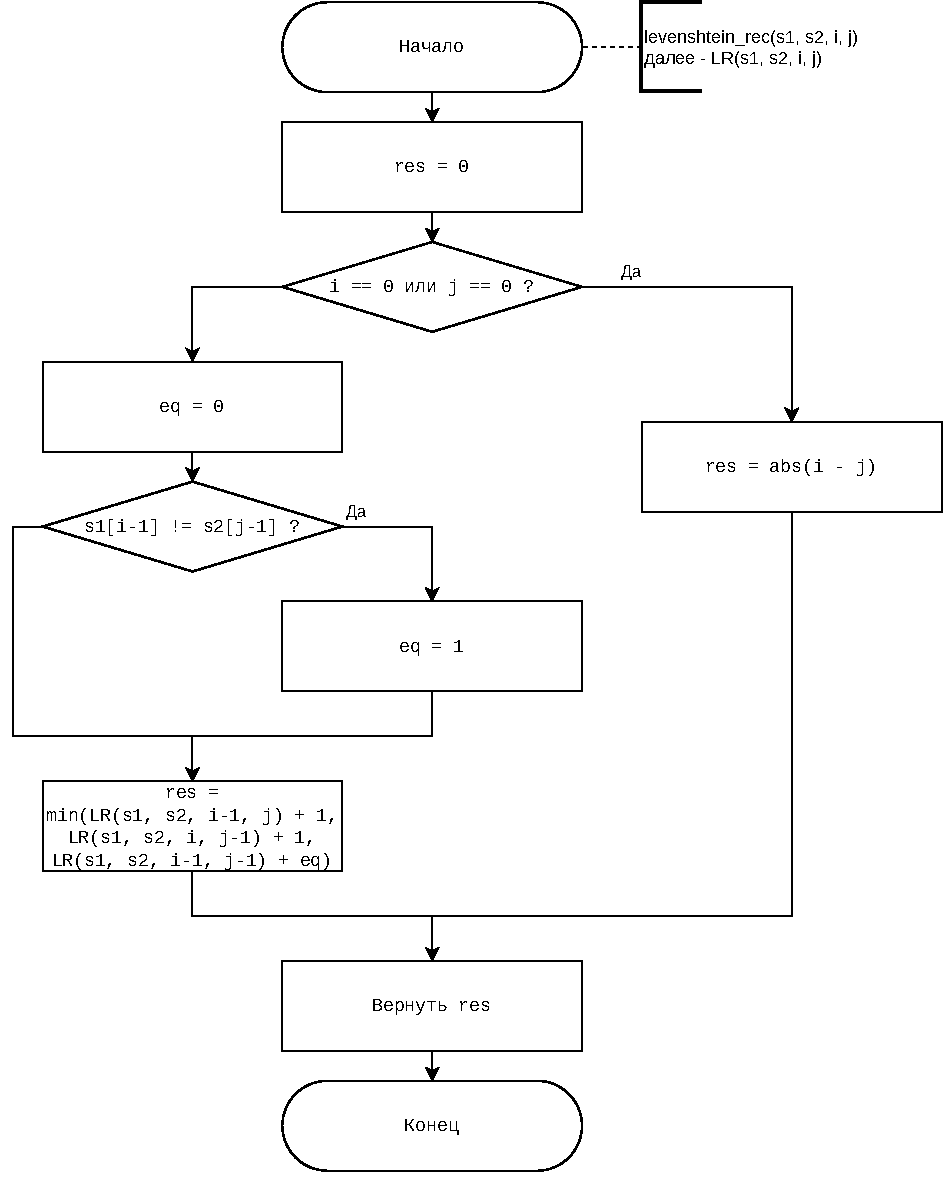
\includegraphics[width=15cm,height=25cm,keepaspectratio]{images/leven_rec.pdf}
            \caption{Рекурсивный алгоритм Левенштейна}
            \label{fig:leven_rec}
        \end{figure}
        
        \begin{figure}
            \centering
            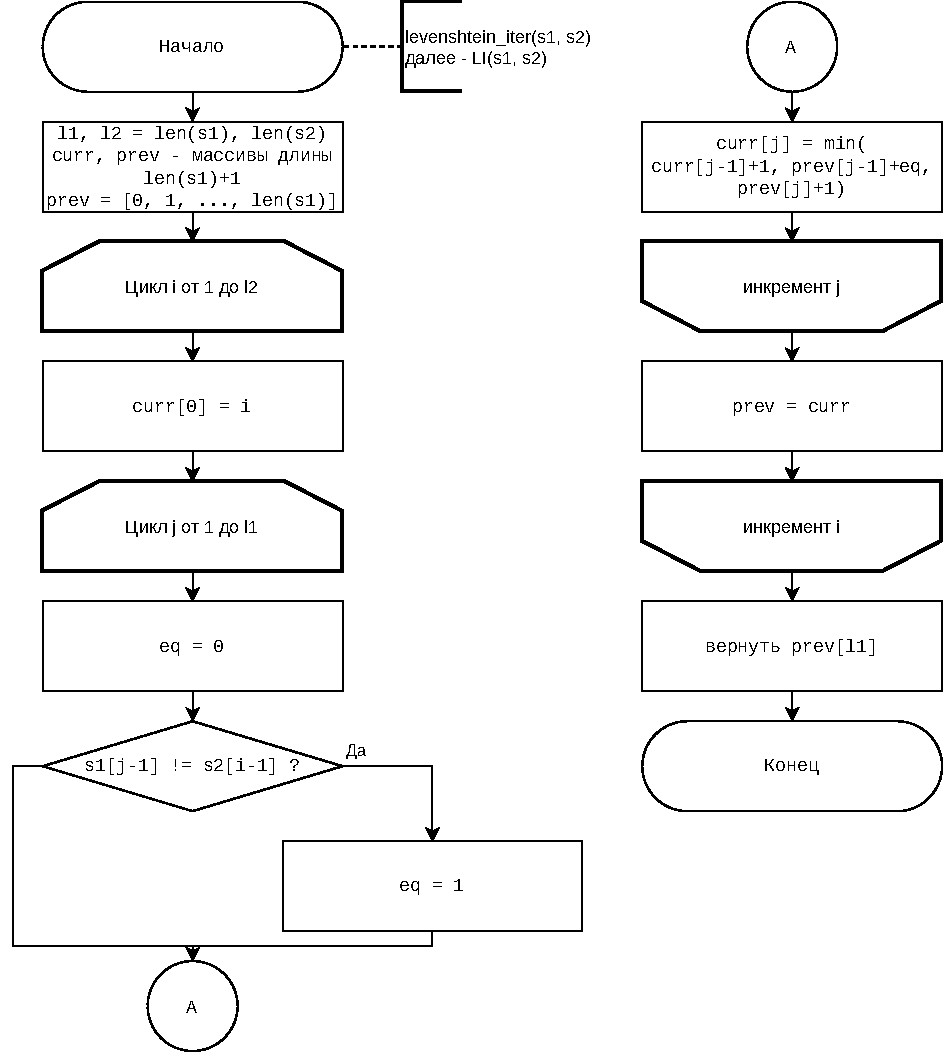
\includegraphics[width=15cm,height=25cm,keepaspectratio]{images/leven_iter.pdf}
            \caption{Рекурсивный алгоритм Левенштейна}
            \label{fig:leven_iter}
        \end{figure}
        
        \begin{figure}
            \centering
            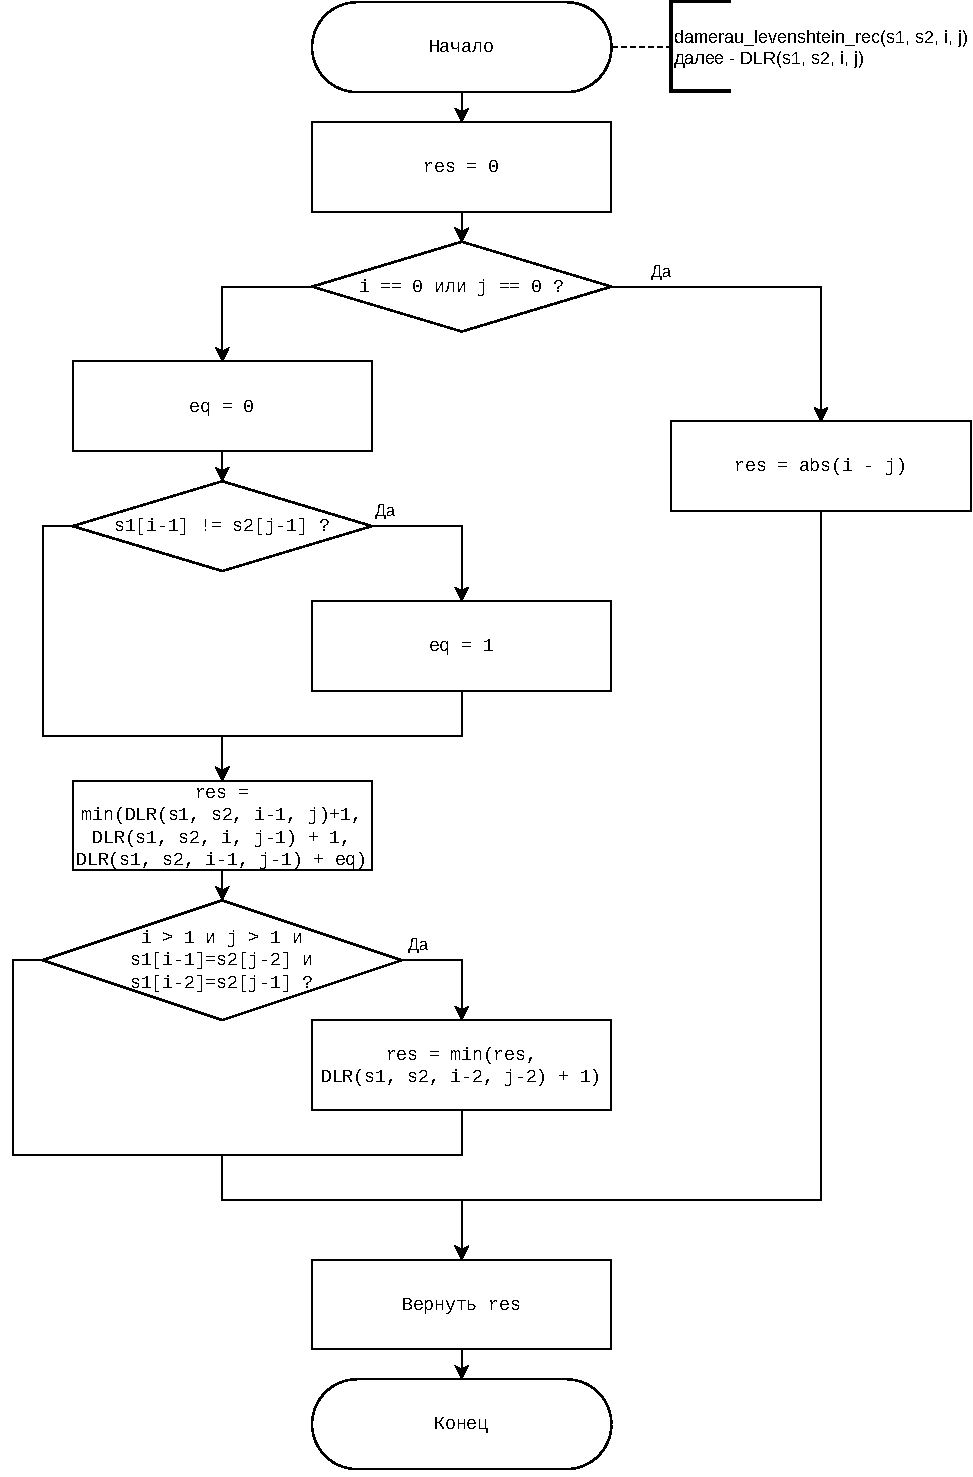
\includegraphics[width=15cm,height=25cm,keepaspectratio]{images/dleven_rec.pdf}
            \caption{Итеративный алгоритм Дамерау - Левенштейна}
            \label{fig:dleven_rec}
        \end{figure}
        
        \begin{figure}
            \centering
            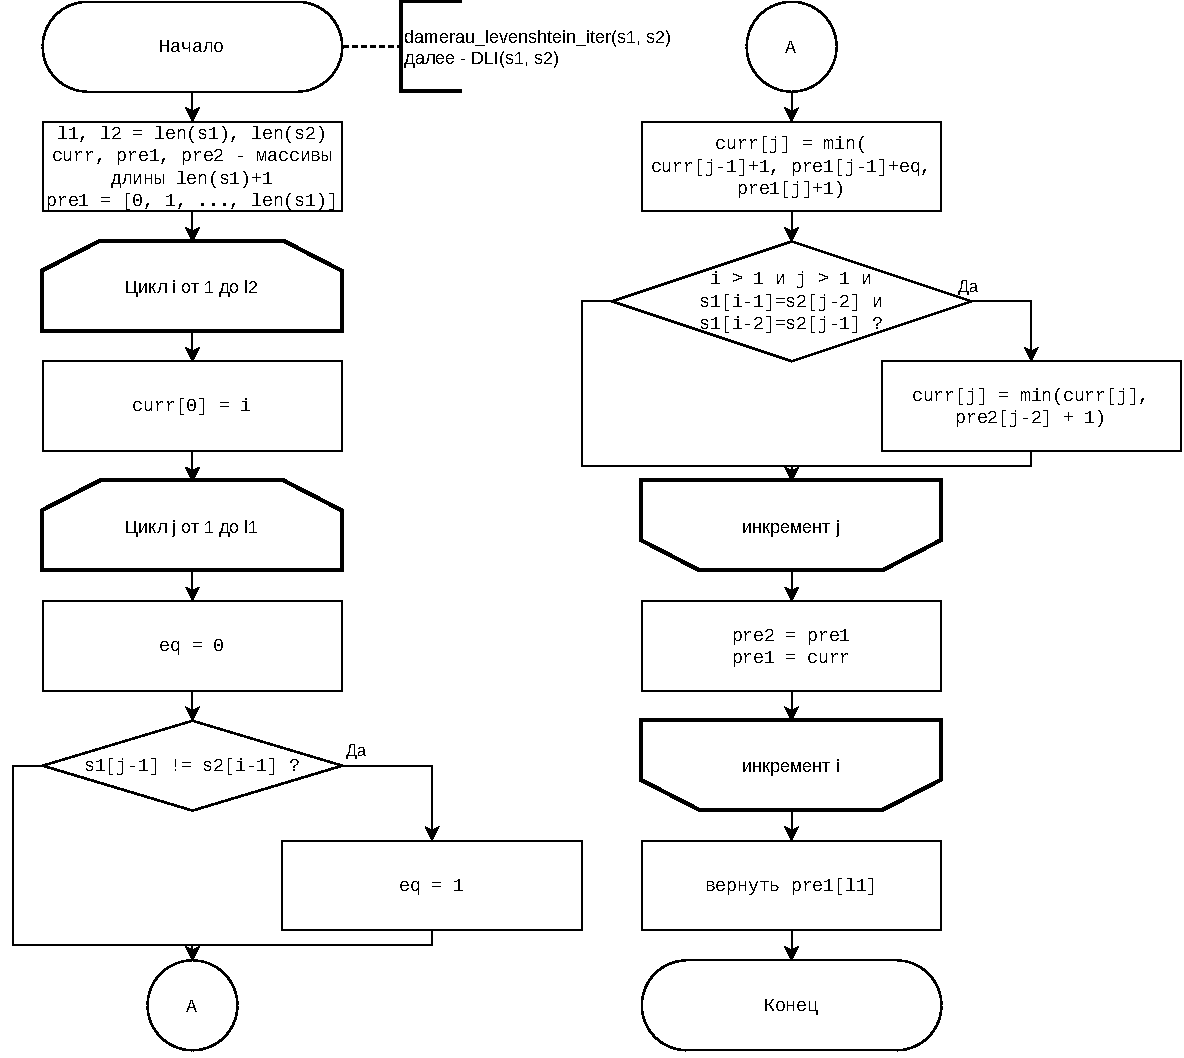
\includegraphics[width=15cm,height=25cm,keepaspectratio]{images/dleven_iter.pdf}
            \caption{Рекурсивный алгоритм Дамерау - Левенштейна}
            \label{fig:dleven_iter}
        \end{figure}
    
    \clearpage

    \section*{Вывод}
    \addcontentsline{toc}{section}{Вывод}
    
        На основе теоретических данных, полученных из аналитического раздела были построены схемы требуемых алгоритмов.